% Options for packages loaded elsewhere
\PassOptionsToPackage{unicode}{hyperref}
\PassOptionsToPackage{hyphens}{url}
%
\documentclass[
]{book}
\title{Probabilidade e Estatística}
\author{Paulo de Souza}
\date{2022-02-23}

\usepackage{amsmath,amssymb}
\usepackage{lmodern}
\usepackage{iftex}
\ifPDFTeX
  \usepackage[T1]{fontenc}
  \usepackage[utf8]{inputenc}
  \usepackage{textcomp} % provide euro and other symbols
\else % if luatex or xetex
  \usepackage{unicode-math}
  \defaultfontfeatures{Scale=MatchLowercase}
  \defaultfontfeatures[\rmfamily]{Ligatures=TeX,Scale=1}
\fi
% Use upquote if available, for straight quotes in verbatim environments
\IfFileExists{upquote.sty}{\usepackage{upquote}}{}
\IfFileExists{microtype.sty}{% use microtype if available
  \usepackage[]{microtype}
  \UseMicrotypeSet[protrusion]{basicmath} % disable protrusion for tt fonts
}{}
\makeatletter
\@ifundefined{KOMAClassName}{% if non-KOMA class
  \IfFileExists{parskip.sty}{%
    \usepackage{parskip}
  }{% else
    \setlength{\parindent}{0pt}
    \setlength{\parskip}{6pt plus 2pt minus 1pt}}
}{% if KOMA class
  \KOMAoptions{parskip=half}}
\makeatother
\usepackage{xcolor}
\IfFileExists{xurl.sty}{\usepackage{xurl}}{} % add URL line breaks if available
\IfFileExists{bookmark.sty}{\usepackage{bookmark}}{\usepackage{hyperref}}
\hypersetup{
  pdftitle={Probabilidade e Estatística},
  pdfauthor={Paulo de Souza},
  hidelinks,
  pdfcreator={LaTeX via pandoc}}
\urlstyle{same} % disable monospaced font for URLs
\usepackage{color}
\usepackage{fancyvrb}
\newcommand{\VerbBar}{|}
\newcommand{\VERB}{\Verb[commandchars=\\\{\}]}
\DefineVerbatimEnvironment{Highlighting}{Verbatim}{commandchars=\\\{\}}
% Add ',fontsize=\small' for more characters per line
\usepackage{framed}
\definecolor{shadecolor}{RGB}{248,248,248}
\newenvironment{Shaded}{\begin{snugshade}}{\end{snugshade}}
\newcommand{\AlertTok}[1]{\textcolor[rgb]{0.94,0.16,0.16}{#1}}
\newcommand{\AnnotationTok}[1]{\textcolor[rgb]{0.56,0.35,0.01}{\textbf{\textit{#1}}}}
\newcommand{\AttributeTok}[1]{\textcolor[rgb]{0.77,0.63,0.00}{#1}}
\newcommand{\BaseNTok}[1]{\textcolor[rgb]{0.00,0.00,0.81}{#1}}
\newcommand{\BuiltInTok}[1]{#1}
\newcommand{\CharTok}[1]{\textcolor[rgb]{0.31,0.60,0.02}{#1}}
\newcommand{\CommentTok}[1]{\textcolor[rgb]{0.56,0.35,0.01}{\textit{#1}}}
\newcommand{\CommentVarTok}[1]{\textcolor[rgb]{0.56,0.35,0.01}{\textbf{\textit{#1}}}}
\newcommand{\ConstantTok}[1]{\textcolor[rgb]{0.00,0.00,0.00}{#1}}
\newcommand{\ControlFlowTok}[1]{\textcolor[rgb]{0.13,0.29,0.53}{\textbf{#1}}}
\newcommand{\DataTypeTok}[1]{\textcolor[rgb]{0.13,0.29,0.53}{#1}}
\newcommand{\DecValTok}[1]{\textcolor[rgb]{0.00,0.00,0.81}{#1}}
\newcommand{\DocumentationTok}[1]{\textcolor[rgb]{0.56,0.35,0.01}{\textbf{\textit{#1}}}}
\newcommand{\ErrorTok}[1]{\textcolor[rgb]{0.64,0.00,0.00}{\textbf{#1}}}
\newcommand{\ExtensionTok}[1]{#1}
\newcommand{\FloatTok}[1]{\textcolor[rgb]{0.00,0.00,0.81}{#1}}
\newcommand{\FunctionTok}[1]{\textcolor[rgb]{0.00,0.00,0.00}{#1}}
\newcommand{\ImportTok}[1]{#1}
\newcommand{\InformationTok}[1]{\textcolor[rgb]{0.56,0.35,0.01}{\textbf{\textit{#1}}}}
\newcommand{\KeywordTok}[1]{\textcolor[rgb]{0.13,0.29,0.53}{\textbf{#1}}}
\newcommand{\NormalTok}[1]{#1}
\newcommand{\OperatorTok}[1]{\textcolor[rgb]{0.81,0.36,0.00}{\textbf{#1}}}
\newcommand{\OtherTok}[1]{\textcolor[rgb]{0.56,0.35,0.01}{#1}}
\newcommand{\PreprocessorTok}[1]{\textcolor[rgb]{0.56,0.35,0.01}{\textit{#1}}}
\newcommand{\RegionMarkerTok}[1]{#1}
\newcommand{\SpecialCharTok}[1]{\textcolor[rgb]{0.00,0.00,0.00}{#1}}
\newcommand{\SpecialStringTok}[1]{\textcolor[rgb]{0.31,0.60,0.02}{#1}}
\newcommand{\StringTok}[1]{\textcolor[rgb]{0.31,0.60,0.02}{#1}}
\newcommand{\VariableTok}[1]{\textcolor[rgb]{0.00,0.00,0.00}{#1}}
\newcommand{\VerbatimStringTok}[1]{\textcolor[rgb]{0.31,0.60,0.02}{#1}}
\newcommand{\WarningTok}[1]{\textcolor[rgb]{0.56,0.35,0.01}{\textbf{\textit{#1}}}}
\usepackage{longtable,booktabs,array}
\usepackage{calc} % for calculating minipage widths
% Correct order of tables after \paragraph or \subparagraph
\usepackage{etoolbox}
\makeatletter
\patchcmd\longtable{\par}{\if@noskipsec\mbox{}\fi\par}{}{}
\makeatother
% Allow footnotes in longtable head/foot
\IfFileExists{footnotehyper.sty}{\usepackage{footnotehyper}}{\usepackage{footnote}}
\makesavenoteenv{longtable}
\usepackage{graphicx}
\makeatletter
\def\maxwidth{\ifdim\Gin@nat@width>\linewidth\linewidth\else\Gin@nat@width\fi}
\def\maxheight{\ifdim\Gin@nat@height>\textheight\textheight\else\Gin@nat@height\fi}
\makeatother
% Scale images if necessary, so that they will not overflow the page
% margins by default, and it is still possible to overwrite the defaults
% using explicit options in \includegraphics[width, height, ...]{}
\setkeys{Gin}{width=\maxwidth,height=\maxheight,keepaspectratio}
% Set default figure placement to htbp
\makeatletter
\def\fps@figure{htbp}
\makeatother
\setlength{\emergencystretch}{3em} % prevent overfull lines
\providecommand{\tightlist}{%
  \setlength{\itemsep}{0pt}\setlength{\parskip}{0pt}}
\setcounter{secnumdepth}{5}
\usepackage{booktabs}
\usepackage[utf8]{inputenc}
\usepackage[brazil]{babel}
\usepackage[top=2cm, bottom = 3cm,left = 2.5cm,right = 2.5cm]{geometry}
\usepackage{xcolor}
%\usepackage{hyperref}


\newtheorem{theorem}{Teorema}
\newtheorem{lemma}[theorem]{Lema}
\newtheorem{example}{Exemplo}
\ifLuaTeX
  \usepackage{selnolig}  % disable illegal ligatures
\fi
\usepackage[]{natbib}
\bibliographystyle{plainnat}

\begin{document}
\maketitle

{
\setcounter{tocdepth}{1}
\tableofcontents
}
\hypertarget{informauxe7uxf5es-gerais}{%
\chapter*{Informações Gerais}\label{informauxe7uxf5es-gerais}}
\addcontentsline{toc}{chapter}{Informações Gerais}

\hypertarget{sobre-o-livro}{%
\section*{Sobre o Livro}\label{sobre-o-livro}}
\addcontentsline{toc}{section}{Sobre o Livro}

Este livro, é apenas um resumo baseado em anotações do autor, com o que diz respeito ao estudo de temas referentes a \textbf{probabilidade} e \textbf{estatística}.

\hypertarget{uso}{%
\section*{Uso}\label{uso}}
\addcontentsline{toc}{section}{Uso}

O livro pode ser usado pelos entusiastas nos assuntos supracitados.

\hypertarget{part-buxe1sico}{%
\part{Básico}\label{part-buxe1sico}}

\hypertarget{introduuxe7uxe3o}{%
\chapter{Introdução}\label{introduuxe7uxe3o}}

\hypertarget{conceitos-principais}{%
\section{Conceitos Principais}\label{conceitos-principais}}

\textbf{Grupos independentes}

\textbf{Grupos pareados}

\textbf{Tipo paramétrico}

\textbf{Tipo não paramétrico}

\hypertarget{testes-de-hipuxf3tese}{%
\section{Testes de Hipótese}\label{testes-de-hipuxf3tese}}

\hypertarget{hipuxf3sete-nula-e-alternativa}{%
\subsection{Hipósete nula e alternativa}\label{hipuxf3sete-nula-e-alternativa}}

\hypertarget{o-significado-de-p-valor}{%
\subsection{O significado de p-valor}\label{o-significado-de-p-valor}}

\hypertarget{testes-de-comparauxe7uxe3o-amostral}{%
\section{Testes de Comparação Amostral}\label{testes-de-comparauxe7uxe3o-amostral}}

São diversos os modelos de dados que são analisados, e cada um destes tem suas características probabilisticas; quando queremos comparar grupos amostrais de nossos dados, são necessários testes para entender melhor como essa amostra se comporta.

Na Tabela abaixo são apresentados alguns dos principais testes de \textbf{Comparação entre Amostras}, cada um dos termos da tabela, assim como os métodos, serão explicados ao longo deste livro/resumo.

\begin{longtable}[]{@{}
  >{\centering\arraybackslash}p{(\columnwidth - 4\tabcolsep) * \real{0.35}}
  >{\centering\arraybackslash}p{(\columnwidth - 4\tabcolsep) * \real{0.21}}
  >{\centering\arraybackslash}p{(\columnwidth - 4\tabcolsep) * \real{0.44}}@{}}
\caption{\label{tab:CompAm} Testes Para Comparação de Amostras}\tabularnewline
\toprule
\begin{minipage}[b]{\linewidth}\centering
\textbf{Quantidade}
\end{minipage} & \begin{minipage}[b]{\linewidth}\centering
\textbf{Tipo}
\end{minipage} & \begin{minipage}[b]{\linewidth}\centering
\textbf{Método de Teste}
\end{minipage} \\
\midrule
\endfirsthead
\toprule
\begin{minipage}[b]{\linewidth}\centering
\textbf{Quantidade}
\end{minipage} & \begin{minipage}[b]{\linewidth}\centering
\textbf{Tipo}
\end{minipage} & \begin{minipage}[b]{\linewidth}\centering
\textbf{Método de Teste}
\end{minipage} \\
\midrule
\endhead
\textbf{2 grupos independentes} & \emph{paramétricos} & Int. e lim. de confiança (1 ou 2 grupos) \\
& & t de Student (1 ou 2 grupos) \\
& & Comparação entre 2 proporções \\
& \emph{não paramétricos} & Qui-quadrado \(\chi^2\) \\
& & U de Mann Whitney \\
& & Prova de Fischer \\
\textbf{2 grupos pareados} & \emph{paramétrico} & t de Student pareado \\
& \emph{não paramétricos} & Prova de MacNemar \\
& & Prova de Wilcoxon \\
\(\geq\) \textbf{3 grupos independentes} & \emph{paramétrico} & ANOVA de 1 ou 2 vias \\
& \emph{não paramétricos} & Qui-quadrado \(\chi^2\) \\
& & Kruskall Wallis \\
\(\geq\) \textbf{3 grupos pareados} & \emph{paramétrico} & ANOVA p/ medidas repetidas \\
& \emph{não paramétrico} & Teste de Friedman \\
\bottomrule
\end{longtable}

Na linha 1 da tabela \ref{tab:CompAm} as abreviações \textbf{Int} e \textbf{lim} significam \textbf{intervalo} e \textbf{limite}, respectivamente.

\hypertarget{estatuxedstica}{%
\chapter{Estatística}\label{estatuxedstica}}

Em probabilidade e estatística, existem diversos conceitos e axiomas que são fundamentais para o entendimento e a resolução dos problemas. Neste capítulo serão desenvolvidos os pontos que serão mais aplicados ao decorrer do livro, demais conceitos que sejam considerados extras, serão apenas indicados e referências para estes são deixadas a disposição.

\hypertarget{conceitos-buxe1sicos-de-estatuxedstica}{%
\section{Conceitos Básicos de Estatística}\label{conceitos-buxe1sicos-de-estatuxedstica}}

Entre os conceitos mais básicos da estatística, estão a \textbf{média, moda} e \textbf{mediana}, de forma direta a explicação de cada uma é dada na sequência

\textbf{Média -} Valor médio\\
\textbf{Mediana -} O valor central\\
\textbf{Moda -} O valor que mais se repete

\hypertarget{muxe9dia}{%
\subsection{Média}\label{muxe9dia}}

A \textbf{média} como citado anteriormente, é o valor médio de uma sequência de dados, matematicamente isso significa a soma de todos os termos, divido pela quantidade dos termos, como apresentado na equação \eqref{eq:media}

\begin{equation}
  \bar{x} = \frac{1}{n} \sum_{i=1}^n x_i
  \label{eq:media}
\end{equation}

Para fixar melhor este conceito, vejamos o exemplo abaixo.

\begin{center}\rule{0.5\linewidth}{0.5pt}\end{center}

\begin{example}
Dado o seguinte registro da velocidade de 13 carros:

\begin{quote}
vel = {[}99,86,87,88,111,86,103,87,94,78,77,85,86{]}
\end{quote}

calcular a média desses dados.

\textbf{Resolução:} Para calcular a média, basta sormamos todos os termos e dividirmos pela quantidade de termos, isto é
\[
\bar{x} = \frac{1}{13}(99+86+87+111+86+103+87+94+78+77+85+86) = 89.77
\]
Portanto, a média das velocidades coletadas é \(\bar{x} = 89.77\)
\end{example}

\begin{center}\rule{0.5\linewidth}{0.5pt}\end{center}

Outro conceito que usualmente aparece, é o de \textbf{média ponderada}, neste caso é associado um determinado `'peso'' a cada um dos termos da amostra.

\hypertarget{mediana}{%
\subsection{Mediana}\label{mediana}}

\hypertarget{moda}{%
\subsection{Moda}\label{moda}}

\hypertarget{variuxe2ncia}{%
\subsection{Variância}\label{variuxe2ncia}}

A \textbf{Variância} é um parâmetro que compara o quão distantes estão os valores de determinado grupo de dados com relação a média deste mesmo grupo. A mesma pode ser do tipo \textbf{Amostral} ou \textbf{Populacional} e a diferença fica mais explicita na equação que as definem.

\begin{equation}
s^2 =  \frac{1}{n-1}\sum_{i=1}^n(x_i - \bar{x})^2
\end{equation}

\hypertarget{desvio-padruxe3o}{%
\subsection{Desvio Padrão}\label{desvio-padruxe3o}}

\hypertarget{probabilidade}{%
\chapter{Probabilidade}\label{probabilidade}}

Neste capítulo serão apresentados os seguintes tópicos:

\begin{itemize}
\tightlist
\item
  Axiomas da Probabilidade
\item
  Análises Combinatórias
\item
  Distribuições de Probabilidade
\end{itemize}

\hypertarget{anuxe1lise-combinatuxf3ria}{%
\section{Análise Combinatória}\label{anuxe1lise-combinatuxf3ria}}

\hypertarget{distribuiuxe7uxf5es-de-probabilidade}{%
\section{Distribuições de Probabilidade}\label{distribuiuxe7uxf5es-de-probabilidade}}

São diversos os tipos de distribuições para análise de dados, podendo ser separado em dois grupos, o de distribuições \textbf{discretas} e o de distribuições \textbf{contínuas}; as mesmas ainda apresentam características importantes, são algumas delas:

\begin{itemize}
\tightlist
\item
  Função de Densidade de Probabilidade (\textbf{PDF})
\item
  Função de Densidade Acumulada (\textbf{CDF})
\item
  Função Percentil (\textbf{PPF})
\item
  Esperança e Variância da Distribuição (\textbf{E(x) e V(x)})
\end{itemize}

Na sequência são apresentadas variás dessas distribuições e suas características, além disso, é disposto implementações em \emph{Octave} para se obter resultados de estudo. Na próxima seção, é feita uma bateria de exemplos que mostram como aquelas são utilizadas.

\hypertarget{normal}{%
\subsection{Normal}\label{normal}}

\hypertarget{densidade-de-probabilidade}{%
\subsubsection*{Densidade de Probabilidade}\label{densidade-de-probabilidade}}
\addcontentsline{toc}{subsubsection}{Densidade de Probabilidade}

A fórmula geral para a \textbf{Função Densidade de Probabilidade} de uma \textbf{Distribuição Normal} é

\begin{equation}
  f(x) =  \frac{1}{\sigma \sqrt{2 \pi}} e^{\frac{-(x-\mu)^2}{(2\sigma^2)}}
\end{equation}

Nos casos em que \(\mu = 0\) e \(\sigma = 1\), temos a chamada \textbf{função normal padrão}, costumeiramente representado por \(N(1,0)\). A equação anterior se reduz a:

\begin{equation}
  f(x) = \frac{1}{\sqrt{2 \pi}} e^{\frac{-x^2}{2}}
\end{equation}

O seguinte gráfico é referente a \textbf{PDF} da normal padrão.

\begin{figure}

{\centering 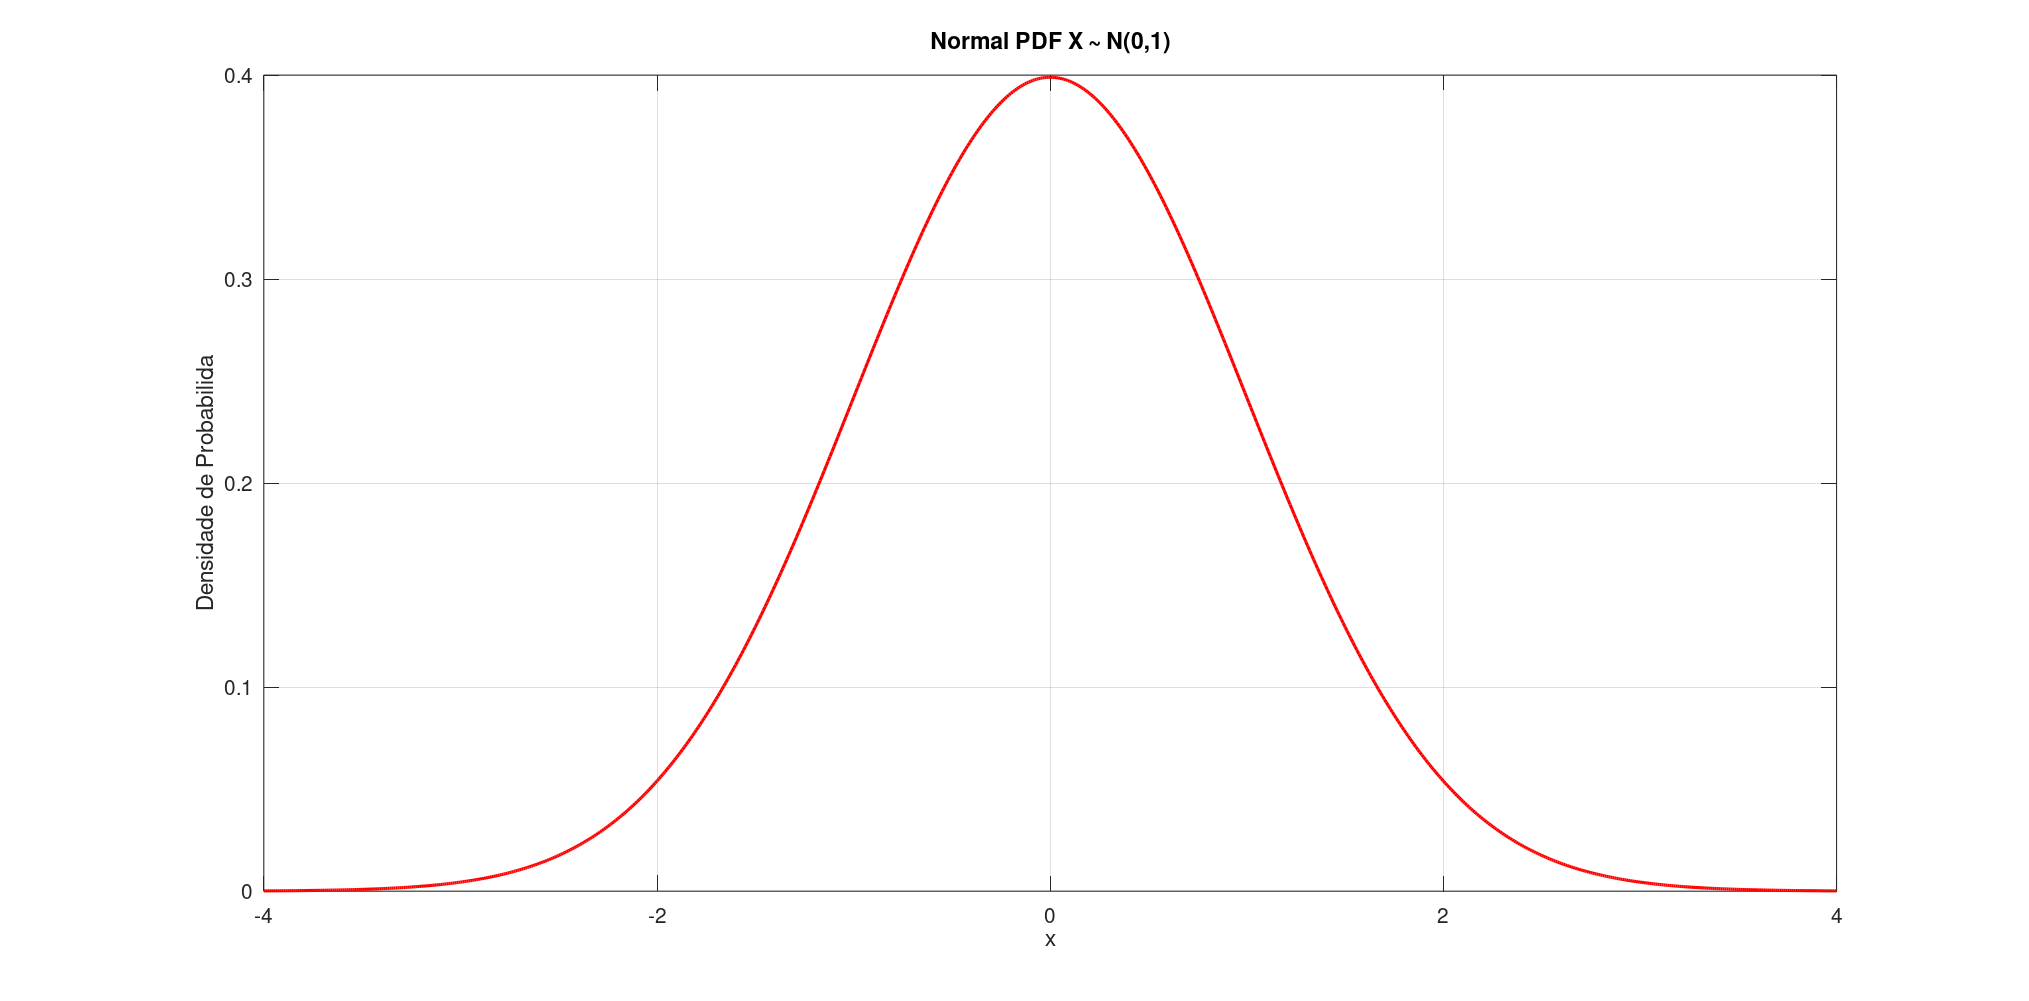
\includegraphics[width=0.5\linewidth]{images/normalpdf} 

}

\caption{Função Densidade de Probabilidade da Normal Padrão}\label{fig:unnamed-chunk-1}
\end{figure}

\hypertarget{densidade-acumulada}{%
\subsubsection*{Densidade Acumulada}\label{densidade-acumulada}}
\addcontentsline{toc}{subsubsection}{Densidade Acumulada}

A fórmula para o cálculo da \textbf{Função Densidade Acumulada} para uma distribuição normal padrão é dado por:

\begin{equation}
  F(x) = \int_{-\infty}^x \frac{1}{\sqrt{2 \pi}} e^{\frac{-x^2}{2}}
\end{equation}

O seguinte gráfico representa os valores de \textbf{CDF} para uma distribuição normal padrão:

\begin{figure}

{\centering 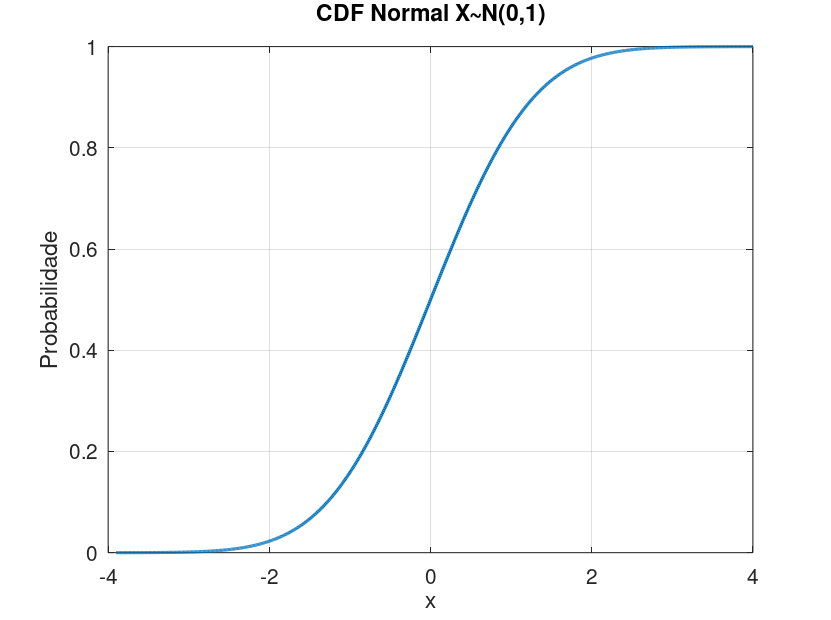
\includegraphics[width=0.5\linewidth]{images/normalcdf} 

}

\caption{Função Densidade Acumulada da Normal Padrão}\label{fig:unnamed-chunk-2}
\end{figure}

\hypertarget{funuxe7uxe3o-percentil}{%
\subsubsection*{Função Percentil}\label{funuxe7uxe3o-percentil}}
\addcontentsline{toc}{subsubsection}{Função Percentil}

Não existe uma forma fechada de se calcular a \textbf{função percentil} para a distribuição normal; no entanto sua interpretação é que dado um valor de probabilidade \(p\) obtêm-se o valor de \(x\), isto é, ela é a inversa da \textbf{CDF}. No gráfico a seguir é apresentada a \textbf{PPF} da distribuição normal padrão.

\begin{figure}

{\centering 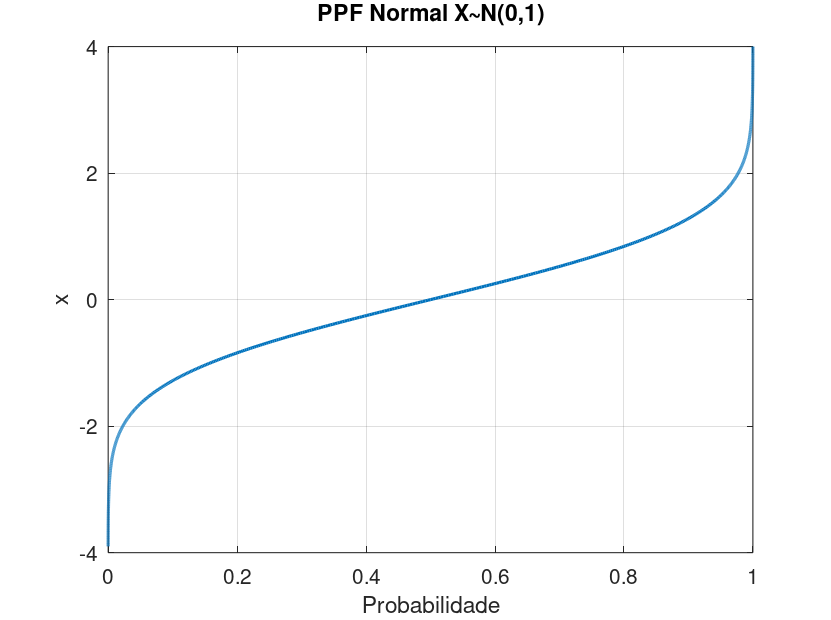
\includegraphics[width=0.5\linewidth]{images/normalppf} 

}

\caption{Função Percentil de Probabilidade da Normal Padrão}\label{fig:unnamed-chunk-3}
\end{figure}

\hypertarget{uniforme}{%
\subsection{Uniforme}\label{uniforme}}

\hypertarget{densidade-de-probabilidade-1}{%
\subsubsection*{Densidade de Probabilidade}\label{densidade-de-probabilidade-1}}
\addcontentsline{toc}{subsubsection}{Densidade de Probabilidade}

A \textbf{Distribuição Uniforme} tem sua \textbf{Densidade de Probabilidade} dada por:

\begin{equation}
f(x) = \frac{1}{B-A} \hspace{2cm} A \leq x \leq B 
\end{equation}

Em que \(A\) é o parâmetro locação (ou desvio) e \(B-A\) é o parâmetro de escala. O gráfico a seguir mostra o caso em que \(A = 1\) e \(B = 3\).

\begin{figure}

{\centering 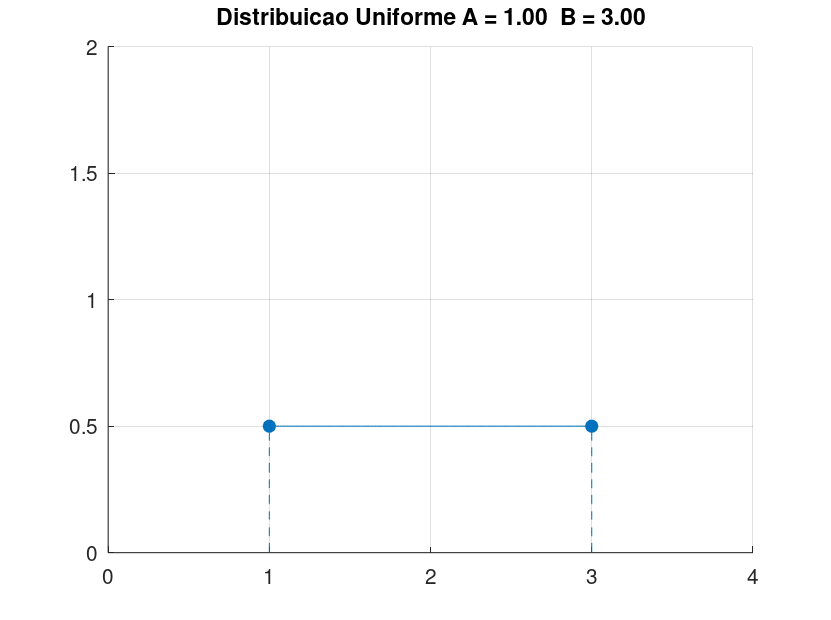
\includegraphics[width=0.5\linewidth]{images/uniformepdf} 

}

\caption{Função Densidade de Probabilidade da Uniforme}\label{fig:unnamed-chunk-4}
\end{figure}

Na ocasião em que \(A = 0\) e \(B = 1\), temos a chamada \textbf{distribuição uniforme padrão}, e a equação anterior se reduz a:

\begin{equation}
f(x) = 1 \hspace{2cm} 0 \leq x \leq 1
\end{equation}

O gráfico a seguir mostra a \textbf{PDF} da uniforme padrão.

\begin{figure}

{\centering 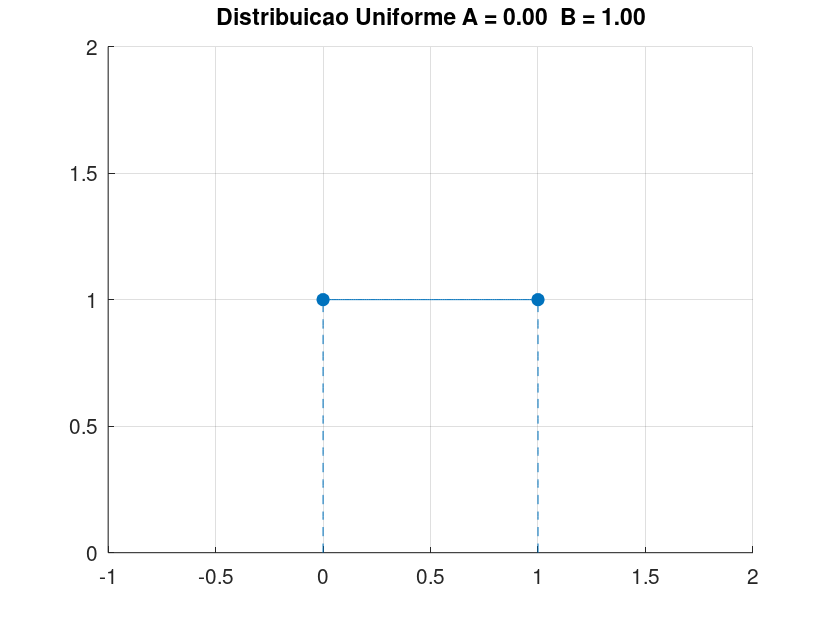
\includegraphics[width=0.5\linewidth]{images/uniformepadraopdf} 

}

\caption{Função Percentil de Probabilidade da Normal Padrão}\label{fig:unnamed-chunk-5}
\end{figure}

\hypertarget{densidade-acumulada-1}{%
\subsubsection*{Densidade Acumulada}\label{densidade-acumulada-1}}
\addcontentsline{toc}{subsubsection}{Densidade Acumulada}

A \textbf{Densidade Acumulada} para um distribuição normal padrão, é simplesmente:
\begin{equation}
  F(x) = x \hspace{2cm} 0 \leq x \leq 1
\end{equation}

O gráfico a seguir apresenta a curva da \textbf{CDF} para a normal padrão.

\hypertarget{funuxe7uxe3o-percentil-1}{%
\subsubsection*{Função Percentil}\label{funuxe7uxe3o-percentil-1}}
\addcontentsline{toc}{subsubsection}{Função Percentil}

A fórmula da \textbf{Função Percentil} para uma distribuição uniforme padrão é bem definida, e é expressa por:

\begin{equation}
  G(p) = p \hspace{2cm} 0 \leq p \leq 1
\end{equation}

O gráfico da \textbf{PPF} da uniforme padrão é apresentado a seguir:

\hypertarget{t-de-student}{%
\subsection{T-de-Student}\label{t-de-student}}

\hypertarget{f-de-fisher---snedecor}{%
\subsection{F de Fisher - Snedecor}\label{f-de-fisher---snedecor}}

\hypertarget{qui---quadrado}{%
\subsection{Qui - Quadrado}\label{qui---quadrado}}

\hypertarget{exponencial}{%
\subsection{Exponencial}\label{exponencial}}

\hypertarget{weidbull}{%
\subsection{Weidbull}\label{weidbull}}

\hypertarget{geomuxe9trica}{%
\subsection{Geométrica}\label{geomuxe9trica}}

\hypertarget{hipergeomuxe9trica}{%
\subsection{Hipergeométrica}\label{hipergeomuxe9trica}}

\hypertarget{gama}{%
\subsection{Gama}\label{gama}}

\hypertarget{beta}{%
\subsection{Beta}\label{beta}}

\hypertarget{bernoulli}{%
\subsection{Bernoulli}\label{bernoulli}}

\hypertarget{binomial}{%
\subsection{Binomial}\label{binomial}}

A \textbf{Distribuição Binomial} é um tipo de distribuição discreta, e uma decorrência dos ensaios de Bernoulli, quando o número de eventos \emph{sucesso} é maior do que 1.

\hypertarget{densidade-de-probabilidade-2}{%
\subsubsection*{Densidade de Probabilidade}\label{densidade-de-probabilidade-2}}
\addcontentsline{toc}{subsubsection}{Densidade de Probabilidade}

O cálculo referente a função \textbf{Densidade de Probabilidade} é dado pela função:

\begin{equation}
  f(x;p,n) = \binom{n}{x} (p)^x (1-p)^{n-x} 
\end{equation}

Em que

\begin{itemize}
\item
  \(x\) é o número de vezes que o meu sucesso deve ocorrer, na ocasião \(x\) é um número inteiro positivo, isto é, \(x = 0, 1, 2, \cdots\);
\item
  \(p\) é a probabilidade do sucesso ocorrer uma única vez;
\item
  \(n\) quantidade de eventos avaliados.
\end{itemize}

Sendo ainda o termo \(\binom{n}{x}\) a \textbf{Combinação} \(C(n,x)\), calculada por:

\[
 C(n,x) = \binom{n}{x} = \frac{n!}{x!(n-x)!}
\]

\hypertarget{densidade-acumulada-2}{%
\subsubsection*{Densidade Acumulada}\label{densidade-acumulada-2}}
\addcontentsline{toc}{subsubsection}{Densidade Acumulada}

\hypertarget{funuxe7uxe3o-percentil-2}{%
\subsubsection*{Função Percentil}\label{funuxe7uxe3o-percentil-2}}
\addcontentsline{toc}{subsubsection}{Função Percentil}

\hypertarget{binomial---negativa}{%
\subsection{Binomial - Negativa}\label{binomial---negativa}}

\hypertarget{poisson}{%
\subsection{Poisson}\label{poisson}}

\hypertarget{densidade-de-probabilidade-3}{%
\subsubsection*{Densidade de Probabilidade}\label{densidade-de-probabilidade-3}}
\addcontentsline{toc}{subsubsection}{Densidade de Probabilidade}

A \textbf{Distribuição de Poisson}, é um tipo de distribuição discreta que tem como função de probabilidade a seguinte equação

\begin{equation}
f(x,\lambda) = \frac{e^{-\lambda} \lambda^x}{x!}
\end{equation}

Em que

\begin{itemize}
\item
  \(x\) é o número de ocorrências no estudo em questão, sendo este ainda um número inteiro não negativo, isto é, \(x = 0, 1, 2, \cdots\);
\item
  \(\lambda\) é o número esperado (médio) de ocorrências no intervalo de estudo.
\end{itemize}

\hypertarget{densidade-acumulada-3}{%
\subsubsection*{Densidade Acumulada}\label{densidade-acumulada-3}}
\addcontentsline{toc}{subsubsection}{Densidade Acumulada}

\hypertarget{funuxe7uxe3o-percentil-3}{%
\subsubsection*{Função Percentil}\label{funuxe7uxe3o-percentil-3}}
\addcontentsline{toc}{subsubsection}{Função Percentil}

\hypertarget{pareto}{%
\subsection{Pareto}\label{pareto}}

\hypertarget{part-testes-amostrais}{%
\part{Testes Amostrais}\label{part-testes-amostrais}}

\hypertarget{dois-grupos-independentes-e-paramuxe9tricos}{%
\chapter{Dois Grupos Independentes e Paramétricos}\label{dois-grupos-independentes-e-paramuxe9tricos}}

\hypertarget{intervalo-e-limite-de-confianuxe7a}{%
\section{Intervalo e limite de confiança}\label{intervalo-e-limite-de-confianuxe7a}}

\hypertarget{t-de-student-1}{%
\section{t de Student}\label{t-de-student-1}}

\hypertarget{comparauxe7uxe3o-entre-2-proporuxe7uxf5es}{%
\section{Comparação entre 2 proporções}\label{comparauxe7uxe3o-entre-2-proporuxe7uxf5es}}

\hypertarget{dois-grupos-independentes-e-nuxe3o-paramuxe9tricos}{%
\chapter{Dois Grupos Independentes e Não-Paramétricos}\label{dois-grupos-independentes-e-nuxe3o-paramuxe9tricos}}

\hypertarget{qui-quadrado}{%
\section{Qui-Quadrado}\label{qui-quadrado}}

\hypertarget{u-de-mann-whitney}{%
\section{U de Mann Whitney}\label{u-de-mann-whitney}}

O teste de \textbf{U de Mann Whitney}, também conhecido como \textbf{Soma do Posto de Wilcoxon} é utilizado na comparação de dois grupos amostrais que tenham preferencialmente o mesmo tamanho.

O método funciona com os seguintes passos:

\begin{enumerate}
\def\labelenumi{\arabic{enumi}.}
\tightlist
\item
  Coloca-se em ordem crescente todos os dados;
\item
  Calcula-se o \textbf{posto} referente a cada um dos valores;
\item
  Atribui-se este posto a cada um dos valores na amostra original;
\item
  Soma-se o posto de cada uma das duas amostras;
\item
  Calcula-se o valor \(U_1\) e \(U_2\), e toma-se \(U = \min(U_1,U_2)\). Define-se as sequintes equações \eqref{eq:U1} e \eqref{eq:U2} para o cálculo de \(U_1\) e \(U_2\):
\end{enumerate}

\begin{equation}
  U_1 = n_1 n_2 + \frac{n_1(n_1+1)}{2} - R_1 
  \label{eq:U1}
\end{equation}

\begin{equation}
U_2 = n_1 n_2 + \frac{n_2(n_2+1)}{2} - R_2
\label{eq:U2}
\end{equation}

\begin{quote}
Caso a quantidade de valores coletados seja menor que 20, isto é, a soma de \(n_1\) e \(n_2\) sejam menores que 20, deve ser feito o comparativo do valor de \(U_{calculado}\) com o valor de \(U_{tabelado}\), consultar a tabela \textbf{Valores Críticos U de Mann-Whitney}\footnote{\href{https://ocw.umb.edu/psychology/psych-270/other-materials/RelativeResourceManager.pdf}{Tabela de Mann Whitney}}.\\
Se a população for maior que 20, é necessário usar a \textbf{tabela z-normal}; nesta ocasião é efetuado mais um passo, que é o cálculo de z.
\end{quote}

\begin{enumerate}
\def\labelenumi{\arabic{enumi}.}
\setcounter{enumi}{5}
\tightlist
\item
  O calculo de \(z\) é dado por:
  \begin{equation}
  z = \frac{U - \mu_R}{\sigma_R}
  \label{eq:zMannWhitney}
  \end{equation}
  em que
  \[ 
  \mu_R = \frac{n_1 \cdot n_2}{2} \hspace{2cm} \sigma_R = \sqrt{\frac{n_1 \cdot n_2(n_1 + n_2 + 1)}{12}}
  \]
\end{enumerate}

Vamos resolver um exemplo, para que fique mais clara a aplicação do método.

\begin{center}\rule{0.5\linewidth}{0.5pt}\end{center}

\begin{example}
Na investigação da eficiência de um novo remédio para asma, um grupo de 10 pacientes aleatórios são submetidos ao teste, sendo metade utilizando o novo remédio e a outra parte um placebo. Após uma semana os mesmos são questionados sobre a quantidade de crises que tiveram durante o período, os dados são apresentados na sequência.

\begin{longtable}[]{@{}cc@{}}
\toprule
\textbf{Placebo} & \textbf{Novo Remédio} \\
\midrule
\endhead
7 & 3 \\
5 & 6 \\
6 & 4 \\
4 & 2 \\
12 & 1 \\
\bottomrule
\end{longtable}

Tome um nível de \(5\%\) de significancia para o teste e as seguintes hipóteses nula e alternativa\\
\(H_0\): A duas populações são iguais\\
\(H_1\): A duas populações não são iguais.

\textbf{Resolução} Vamos tomar como \textbf{Pl} a coluna do \textbf{Placebo} e \textbf{NR} a coluna do \textbf{Novo Remédio}, então \(n_{Pl} = 5\) e \(n_{NR} = 5\); seguindo o passo a passo do método, iremos primeiro colocar todos os dados em ordem crescente, então fazemos:

\textbf{Passo 1} Colocando todos os dados em ordem crescente

\begin{longtable}[]{@{}cllllllllll@{}}
\toprule
\# ordem & 1 & 2 & 3 & 4 & 4 & 5 & 6 & 6 & 7 & 12 \\
\midrule
\endhead
\bottomrule
\end{longtable}

\textbf{Passo 2} Deve ser calculado o posto de cada valor; o posto de uma amostra é dado de acordo com a posição na qual os dados de mesmo valor estão localizados na sequência crescente e a quantidade dos mesmos. Por exemplo, na ocasião o primeiro valor repetido é o número 4, o mesmo está localizado na posição 4 e 5 (sendo então duas repetições) da lista ordenada, então o posto do valor 4 será
\[
\text{posto}_4 = \frac{4+5}{2} = 4.5
\]
o mesmo procedimento é feito para o valor 6, que se encontra na posição 7 e 8, logo:
\[
\text{posto}_6 = \frac{7+8}{2} = 7.5
\]
os demais valores irão assumir os postos de suas posições, sendo assim:

\begin{longtable}[]{@{}lcccccccccc@{}}
\toprule
\textbf{\# ordem} & \textbf{1} & \textbf{2} & \textbf{3} & \textbf{4} & \textbf{4} & \textbf{5} & \textbf{6} & \textbf{6} & \textbf{7} & \textbf{12} \\
\midrule
\endhead
\textbf{\# postos} & \textbf{1} & \textbf{2} & \textbf{3} & \textbf{4.5} & \textbf{4.5} & \textbf{6} & \textbf{7.5} & \textbf{7.5} & \textbf{9} & \textbf{10} \\
\bottomrule
\end{longtable}

\textbf{Passo 3} Agora deve-se atribuir o valor dos postos encontrados, em cada uma das amostras originais

\begin{longtable}[]{@{}cccc@{}}
\toprule
\textbf{Placebo} & \textbf{Posto Pl} & \textbf{Novo Remédio} & \textbf{Posto NR} \\
\midrule
\endhead
7 & 9 & 3 & 3 \\
5 & 6 & 6 & 7.5 \\
6 & 7.5 & 4 & 4.5 \\
4 & 4.5 & 2 & 2 \\
12 & 10 & 1 & 1 \\
\bottomrule
\end{longtable}

\textbf{Passo 4} Agora somaremos o posto de cada uma das amostras
\[
R_{Pl} = 9 + 6 + 7.5 + 4.5 + 10 = 37\\
R_{NR} = 3 + 7.5 + 4.5 + 2 + 1 = 18
\]

\textbf{Passo 5} Iremos calcular o valor de U, o que segue:

Primeiro \(U_{Pl}\)
\[
U_{Pl} = n_{Pl} \cdot n_{NR} + \frac{n_{Pl}(n_{Pl}+1)}{2} - R_{Pl} \hspace{1cm} \therefore 
\]
\[
U_{Pl} = 5 \cdot 5 + \frac{5(5+1)}{2} - 37 \hspace{.5cm} \Rightarrow \hspace{.5cm} U_{Pl} = 3 
\]

e agora \(U_{NR}\)
\[
U_{NR} = n_{Pl} \cdot n_{NR} + \frac{n_{NR}(n_{NR}+1)}{2} - R_{NR} \hspace{1cm} \therefore 
\]

\[
U_{NR} = 5 \cdot 5 + \frac{5(5+1)}{2} - 18 \hspace{.5cm} \Rightarrow \hspace{.5cm} U_{NR} = 22 
\]
Com ambos os valores calculados, tomaremos o menor, sendo assim \(U = 3\), como a amostra só tem 10 valores, podemos então olhar a tabela de valor critíco U de Mann Whitney, uma parte da mesma é apresentada na figura a seguir

\begin{figure}

{\centering 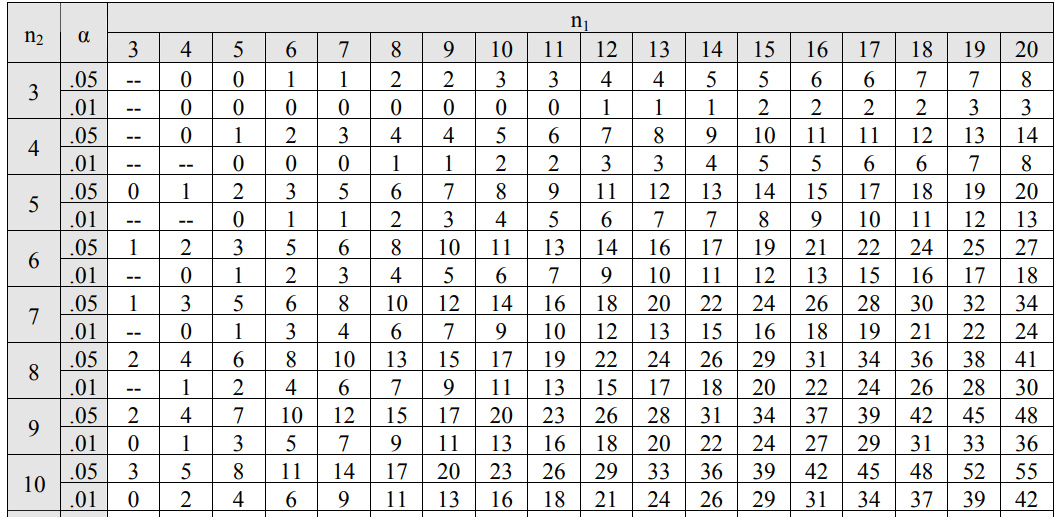
\includegraphics[width=0.7\linewidth]{images/TabelaCriticalU} 

}

\caption{Parte da Tabela de Valores Críticos de U}\label{fig:unnamed-chunk-6}
\end{figure}

Como nosso \(n_1 = 5, \ n_2 = 5\) e \(\alpha = 5\%\), temos \(U_{tabelado} = 2\); sendo o U calculado maior que o tabelado, \(2 < 3\), então a hipótese nula é aceita.
\end{example}

\begin{center}\rule{0.5\linewidth}{0.5pt}\end{center}

\textbf{OBS:} O exercício foi retirado e adaptado do site \href{https://sphweb.bumc.bu.edu/otlt/mph-modules/bs/bs704_nonparametric/bs704_nonparametric4.html}{Mann-Whitney}

Para automatizar o problema foi criada uma função em \emph{Octave} na qual é apresentada na sequência

\begin{Shaded}
\begin{Highlighting}[]
\ControlFlowTok{function}\NormalTok{ testeU\_MannWhitney(A}\OperatorTok{,}\NormalTok{B)}

\FunctionTok{display}\NormalTok{(}\StringTok{\textquotesingle{}Dados fornecidos\textquotesingle{}}\NormalTok{)}
\FunctionTok{display}\NormalTok{(A)}
\FunctionTok{display}\NormalTok{(B)}

\NormalTok{nA }\OperatorTok{=} \FunctionTok{length}\NormalTok{(A)}\OperatorTok{;}   \CommentTok{\%quantidade de observacoes em A}
\NormalTok{nB }\OperatorTok{=} \FunctionTok{length}\NormalTok{(B)}\OperatorTok{;}   \CommentTok{\%quantidade de observacoes em B}

\NormalTok{n }\OperatorTok{=}\NormalTok{ nA}\OperatorTok{+}\NormalTok{nB}\OperatorTok{;}        \CommentTok{\%quantidade de observacoes totais}

\NormalTok{C }\OperatorTok{=}\NormalTok{ [A}\OperatorTok{,}\NormalTok{B]}\OperatorTok{;}        \CommentTok{\%vetor auxiliar}
\NormalTok{C\_cres }\OperatorTok{=} \FunctionTok{sort}\NormalTok{(C)}\OperatorTok{;} \CommentTok{\%vetor auxiliar em ordem crescente}

\CommentTok{\%Pesos em A}
\ControlFlowTok{for}\NormalTok{ k}\OperatorTok{=}\FloatTok{1}\OperatorTok{:}\NormalTok{nA}
\NormalTok{  mA }\OperatorTok{=} \FunctionTok{find}\NormalTok{(C\_cres }\OperatorTok{==}\NormalTok{ A(k))}\OperatorTok{;}
\NormalTok{  pesoA(k) }\OperatorTok{=} \FunctionTok{sum}\NormalTok{(mA)}\OperatorTok{/}\FunctionTok{length}\NormalTok{(mA)}\OperatorTok{;}
\ControlFlowTok{end}

\NormalTok{RA }\OperatorTok{=} \FunctionTok{sum}\NormalTok{(pesoA)}\OperatorTok{;}

\CommentTok{\%Pesos em B}
\ControlFlowTok{for}\NormalTok{ k}\OperatorTok{=}\FloatTok{1}\OperatorTok{:}\NormalTok{nB}
\NormalTok{  mB }\OperatorTok{=} \FunctionTok{find}\NormalTok{(C\_cres }\OperatorTok{==}\NormalTok{ B(k))}\OperatorTok{;}
\NormalTok{  pesoB(k) }\OperatorTok{=} \FunctionTok{sum}\NormalTok{(mB)}\OperatorTok{/}\FunctionTok{length}\NormalTok{(mB)}\OperatorTok{;}
\ControlFlowTok{end}

\NormalTok{RB }\OperatorTok{=} \FunctionTok{sum}\NormalTok{(pesoB)}\OperatorTok{;}

\ControlFlowTok{for}\NormalTok{ k}\OperatorTok{=}\FloatTok{1}\OperatorTok{:}\NormalTok{nA}
  \ControlFlowTok{if}\NormalTok{ k }\OperatorTok{==} \FloatTok{1}
    \FunctionTok{fprintf}\NormalTok{(}\StringTok{\textquotesingle{}Valor A           rankA\textbackslash{}n\textquotesingle{}}\NormalTok{)}
  \ControlFlowTok{end}
  \FunctionTok{fprintf}\NormalTok{(}\StringTok{\textquotesingle{}\%7.2f     \%10.2f\textbackslash{}n\textquotesingle{}}\OperatorTok{,}\NormalTok{A(k)}\OperatorTok{,}\NormalTok{pesoA(k))}
  \ControlFlowTok{if}\NormalTok{ k}\OperatorTok{==}\NormalTok{nA}
    \FunctionTok{fprintf}\NormalTok{(}\StringTok{\textquotesingle{}nA = \%4.2f     RA = \%5.2f\textbackslash{}n\textbackslash{}n\textquotesingle{}}\OperatorTok{,}\NormalTok{nA}\OperatorTok{,}\NormalTok{RA)}
  \ControlFlowTok{end}
\ControlFlowTok{end}

\ControlFlowTok{for}\NormalTok{ k}\OperatorTok{=}\FloatTok{1}\OperatorTok{:}\NormalTok{nB}
  \ControlFlowTok{if}\NormalTok{ k }\OperatorTok{==} \FloatTok{1}
    \FunctionTok{fprintf}\NormalTok{(}\StringTok{\textquotesingle{}Valor B           rankB\textbackslash{}n\textquotesingle{}}\NormalTok{)}
  \ControlFlowTok{end}
  \FunctionTok{fprintf}\NormalTok{(}\StringTok{\textquotesingle{}\%7.2f     \%10.2f\textbackslash{}n\textquotesingle{}}\OperatorTok{,}\NormalTok{B(k)}\OperatorTok{,}\NormalTok{pesoB(k))}
  \ControlFlowTok{if}\NormalTok{ k}\OperatorTok{==}\NormalTok{nB}
    \FunctionTok{fprintf}\NormalTok{(}\StringTok{\textquotesingle{}nB = \%4.2f     RB = \%5.2f\textbackslash{}n\textbackslash{}n\textquotesingle{}}\OperatorTok{,}\NormalTok{nB}\OperatorTok{,}\NormalTok{RB)}
  \ControlFlowTok{end}
\ControlFlowTok{end}

\CommentTok{\%Estatistica para o teste de Mann Whitney}
\NormalTok{UA }\OperatorTok{=}\NormalTok{ nA}\OperatorTok{*}\NormalTok{nB }\OperatorTok{+} \FloatTok{0.5}\OperatorTok{*}\NormalTok{(nA}\OperatorTok{*}\NormalTok{(nA}\OperatorTok{+}\FloatTok{1}\NormalTok{))}\OperatorTok{{-}}\NormalTok{RA}\OperatorTok{;}
\NormalTok{UB }\OperatorTok{=}\NormalTok{ nA}\OperatorTok{*}\NormalTok{nB }\OperatorTok{+} \FloatTok{0.5}\OperatorTok{*}\NormalTok{(nB}\OperatorTok{*}\NormalTok{(nB}\OperatorTok{+}\FloatTok{1}\NormalTok{))}\OperatorTok{{-}}\NormalTok{RB}\OperatorTok{;}
\FunctionTok{fprintf}\NormalTok{(}\StringTok{\textquotesingle{}UA = \%.2f   UB = \%.2f\textbackslash{}n\textquotesingle{}}\OperatorTok{,}\NormalTok{UA}\OperatorTok{,}\NormalTok{UB)}
\NormalTok{U }\OperatorTok{=} \FunctionTok{min}\NormalTok{(UA}\OperatorTok{,}\NormalTok{UB)}\OperatorTok{;}

\CommentTok{\%Para n\textgreater{}20 usa{-}se a tabela da distribuicao normal}
\ControlFlowTok{if}\NormalTok{ n}\OperatorTok{\textgreater{}}\FloatTok{20}
  \FunctionTok{display}\NormalTok{(}\StringTok{\textquotesingle{}Use a Tabela normal\textquotesingle{}}\NormalTok{)}
\NormalTok{  mu\_r }\OperatorTok{=}\NormalTok{ nA}\OperatorTok{*}\NormalTok{nB}\OperatorTok{/}\FloatTok{2}\OperatorTok{;}
\NormalTok{  sig\_r }\OperatorTok{=} \FunctionTok{sqrt}\NormalTok{((nA}\OperatorTok{*}\NormalTok{nB)}\OperatorTok{*}\NormalTok{(nA}\OperatorTok{+}\NormalTok{nB}\OperatorTok{+}\FloatTok{1}\NormalTok{)}\OperatorTok{/}\FloatTok{12}\NormalTok{)}\OperatorTok{;}
\NormalTok{  z }\OperatorTok{=}\NormalTok{ (U}\OperatorTok{{-}}\NormalTok{mu\_r)}\OperatorTok{/}\NormalTok{sig\_r}
  
\CommentTok{\%Para n\textless{}=20 usa{-}se a tabela de Valores Criticos de Mann{-}Whitney}
\ControlFlowTok{else}
  \FunctionTok{display}\NormalTok{(}\StringTok{\textquotesingle{}Use a Tabela de Mann{-}Whitney\textquotesingle{}}\NormalTok{)}
  \FunctionTok{fprintf}\NormalTok{(}\StringTok{\textquotesingle{}Sendo o valor calculado de U = \%.2f\textbackslash{}n\textquotesingle{}}\OperatorTok{,}\NormalTok{U)}
\ControlFlowTok{end}
\end{Highlighting}
\end{Shaded}

Para o nosso exemplo então podemos definir \texttt{Pl\ =\ {[}7\ 5\ 6\ 4\ 12{]}}, \texttt{NR\ =\ {[}3\ 6\ 4\ 2\ 1{]}} e usar o comando \texttt{testeU\_MannWhitney(Pl,NR)}, o resultado obtido é apresentado na sequência

\begin{verbatim}
## Dados fornecidos
## A =
## 
##     7    5    6    4   12
## 
## B =
## 
##    3   6   4   2   1
## 
## Valor A           rankA
##    7.00           9.00
##    5.00           6.00
##    6.00           7.50
##    4.00           4.50
##   12.00          10.00
## nA = 5.00     RA = 37.00
## 
## Valor B           rankB
##    3.00           3.00
##    6.00           7.50
##    4.00           4.50
##    2.00           2.00
##    1.00           1.00
## nB = 5.00     RB = 18.00
## 
## UA = 3.00   UB = 22.00
## Use a Tabela de Mann-Whitney
## Sendo o valor calculado de U = 3.00
\end{verbatim}

\hypertarget{prova-de-fischer}{%
\section{Prova de Fischer}\label{prova-de-fischer}}

\hypertarget{dois-grupos-pareados-e-paramuxe9tricos}{%
\chapter{Dois grupos Pareados e Paramétricos}\label{dois-grupos-pareados-e-paramuxe9tricos}}

\hypertarget{teste-de-t-student-pareado}{%
\section{Teste de t-Student pareado}\label{teste-de-t-student-pareado}}

\hypertarget{dois-grupos-pareados-e-nuxe3o---paramuxe9tricos}{%
\chapter{Dois grupos Pareados e Não - Paramétricos}\label{dois-grupos-pareados-e-nuxe3o---paramuxe9tricos}}

\hypertarget{prova-de-macnemar}{%
\section{Prova de MacNemar}\label{prova-de-macnemar}}

\hypertarget{prova-de-wilcoxon}{%
\section{Prova de Wilcoxon}\label{prova-de-wilcoxon}}

\hypertarget{truxeas-ou-mais-grupos-independentes-e-paramuxe9tricos}{%
\chapter{Três ou mais grupos Independentes e Paramétricos}\label{truxeas-ou-mais-grupos-independentes-e-paramuxe9tricos}}

\hypertarget{teste-de-tuckey}{%
\section{Teste de Tuckey}\label{teste-de-tuckey}}

\hypertarget{anova-de-1-ou-2-vias}{%
\section{ANOVA de 1 ou 2 vias}\label{anova-de-1-ou-2-vias}}

\hypertarget{part-testes-de-normalidade}{%
\part{Testes de Normalidade}\label{part-testes-de-normalidade}}

\hypertarget{testes-de-normalidade}{%
\chapter{Testes de Normalidade}\label{testes-de-normalidade}}

\hypertarget{shapiro-wilk}{%
\section{Shapiro-Wilk}\label{shapiro-wilk}}

\hypertarget{kolmogorov---smirnov}{%
\section{Kolmogorov - Smirnov}\label{kolmogorov---smirnov}}

\hypertarget{anderson---darling}{%
\section{Anderson - Darling}\label{anderson---darling}}

\hypertarget{cramer-von-mises}{%
\section{Cramer Von-Mises}\label{cramer-von-mises}}

\hypertarget{part-aca}{%
\part{ACA}\label{part-aca}}

\hypertarget{anuxe1lise-de-concorduxe2ncia-de-atributos}{%
\chapter{Análise de Concordância de Atributos}\label{anuxe1lise-de-concorduxe2ncia-de-atributos}}

\hypertarget{estuxe1tica-kappa}{%
\chapter{Estática Kappa}\label{estuxe1tica-kappa}}

\hypertarget{teste-kappa-de-cohen}{%
\section{Teste Kappa de Cohen}\label{teste-kappa-de-cohen}}

\hypertarget{teste-kappa-de-fleiss}{%
\section{Teste Kappa de Fleiss}\label{teste-kappa-de-fleiss}}

  \bibliography{book.bib,packages.bib}

\end{document}
